\documentclass[8pt,aspectratio=169]{beamer}
\usetheme{Madrid}
\usepackage{graphicx}
\usepackage{booktabs}
\usepackage{adjustbox}
\usepackage{multicol}
\usepackage{amsmath}
\usepackage{listings}
\usepackage{xcolor}

% Color definitions
\definecolor{mlblue}{RGB}{0,102,204}
\definecolor{mlpurple}{RGB}{51,51,178}
\definecolor{mllavender}{RGB}{173,173,224}
\definecolor{mllavender2}{RGB}{193,193,232}
\definecolor{mllavender3}{RGB}{204,204,235}
\definecolor{mllavender4}{RGB}{214,214,239}
\definecolor{mlorange}{RGB}{255, 127, 14}
\definecolor{mlgreen}{RGB}{44, 160, 44}
\definecolor{mlred}{RGB}{214, 39, 40}
\definecolor{mlgray}{RGB}{127, 127, 127}

% Additional colors
\definecolor{lightgray}{RGB}{240, 240, 240}
\definecolor{midgray}{RGB}{180, 180, 180}

% Apply custom colors to Madrid theme
\setbeamercolor{palette primary}{bg=mllavender3,fg=mlpurple}
\setbeamercolor{palette secondary}{bg=mllavender2,fg=mlpurple}
\setbeamercolor{palette tertiary}{bg=mllavender,fg=white}
\setbeamercolor{palette quaternary}{bg=mlpurple,fg=white}

\setbeamercolor{structure}{fg=mlpurple}
\setbeamercolor{section in toc}{fg=mlpurple}
\setbeamercolor{subsection in toc}{fg=mlblue}
\setbeamercolor{title}{fg=mlpurple}
\setbeamercolor{frametitle}{fg=mlpurple,bg=mllavender3}
\setbeamercolor{block title}{bg=mllavender2,fg=mlpurple}
\setbeamercolor{block body}{bg=mllavender4,fg=black}

% Remove navigation symbols
\setbeamertemplate{navigation symbols}{}

% Clean itemize/enumerate
\setbeamertemplate{itemize items}[circle]
\setbeamertemplate{enumerate items}[default]

% Reduce margins
\setbeamersize{text margin left=5mm,text margin right=5mm}

% Bottom note command
\newcommand{\bottomnote}[1]{%
\vfill
\vspace{-2mm}
\textcolor{mllavender2}{\rule{\textwidth}{0.4pt}}
\vspace{1mm}
\footnotesize
\textbf{#1}
}

% Code listing style
\lstset{
    basicstyle=\tiny\ttfamily,
    keywordstyle=\color{mlblue},
    commentstyle=\color{mlgray},
    stringstyle=\color{mlgreen},
    breaklines=true,
    frame=none,
    backgroundcolor=\color{lightgray},
    showstringspaces=false
}

\title{Sentence Embeddings with Hugging Face}
\subtitle{From Text to Numbers: Understanding Semantic Representations}
\author{NLP Tutorial Series}
\institute{BSc Level - Natural Language Processing}
\date{\today}

\begin{document}

% ==================== TITLE SLIDE ====================
\begin{frame}[plain]
\vspace{1.5cm}
\begin{center}
{\Huge\textbf{Sentence Embeddings with Hugging Face}}\\[0.5cm]
{\Large From Text to Numbers: Understanding Semantic Representations}\\[2cm]
{\normalsize BSc Level Tutorial}\\[0.3cm]
{\normalsize Natural Language Processing}
\end{center}
\end{frame}

% ==================== LEARNING OBJECTIVES ====================
\begin{frame}[t]{Learning Objectives}

By the end of this tutorial, you will be able to:

\vspace{0.5cm}

\begin{enumerate}
    \item Understand what sentence embeddings are and why they are useful
    \item Use the \texttt{sentence-transformers} library from Hugging Face
    \item Generate embeddings with \texttt{SentenceTransformer('all-MiniLM-L6-v2')}
    \item Calculate and interpret cosine similarity between sentences
    \item Visualize high-dimensional embeddings using PCA and t-SNE
    \item Apply embeddings to practical NLP tasks (search, clustering)
\end{enumerate}

\bottomnote{Prerequisite: Basic Python, basic linear algebra (vectors, dot products)}
\end{frame}

% ==================== SECTION: INTRODUCTION ====================
\section{Introduction \& Motivation}

\begin{frame}[t]{The Problem: How Do Computers Understand Text?}

\begin{columns}[t]
\begin{column}{0.48\textwidth}
\textbf{Traditional Approaches}
\begin{itemize}
    \item \textbf{Bag of Words}: Count word frequencies
    \item \textbf{One-Hot Encoding}: Binary vectors
    \item \textbf{TF-IDF}: Weighted term frequencies
\end{itemize}

\vspace{0.5cm}
\textbf{Limitations:}
\begin{itemize}
    \item No semantic understanding
    \item Sparse, high-dimensional
    \item Cannot capture synonyms
    \item ``King'' and ``Queen'' are equally distant as ``King'' and ``Table''
\end{itemize}
\end{column}

\begin{column}{0.48\textwidth}
\textbf{Modern Approach: Embeddings}
\begin{itemize}
    \item \textbf{Dense vectors}: Continuous representations
    \item \textbf{Semantic meaning}: Similar meanings → Similar vectors
    \item \textbf{Fixed dimension}: Same size for any text
\end{itemize}

\vspace{0.5cm}
\textbf{Advantages:}
\begin{itemize}
    \item Captures semantic relationships
    \item Dense, efficient representations
    \item Similar words/sentences cluster together
    \item ``King'' and ``Queen'' are close, far from ``Table''
\end{itemize}
\end{column}
\end{columns}

\bottomnote{Transition: From discrete symbols to continuous meaning vectors}
\end{frame}

% ==================== SECTION: CONCEPTS ====================
\section{Core Concepts}

\begin{frame}[t]{What Are Embeddings?}

\vspace{0.3cm}

\begin{center}
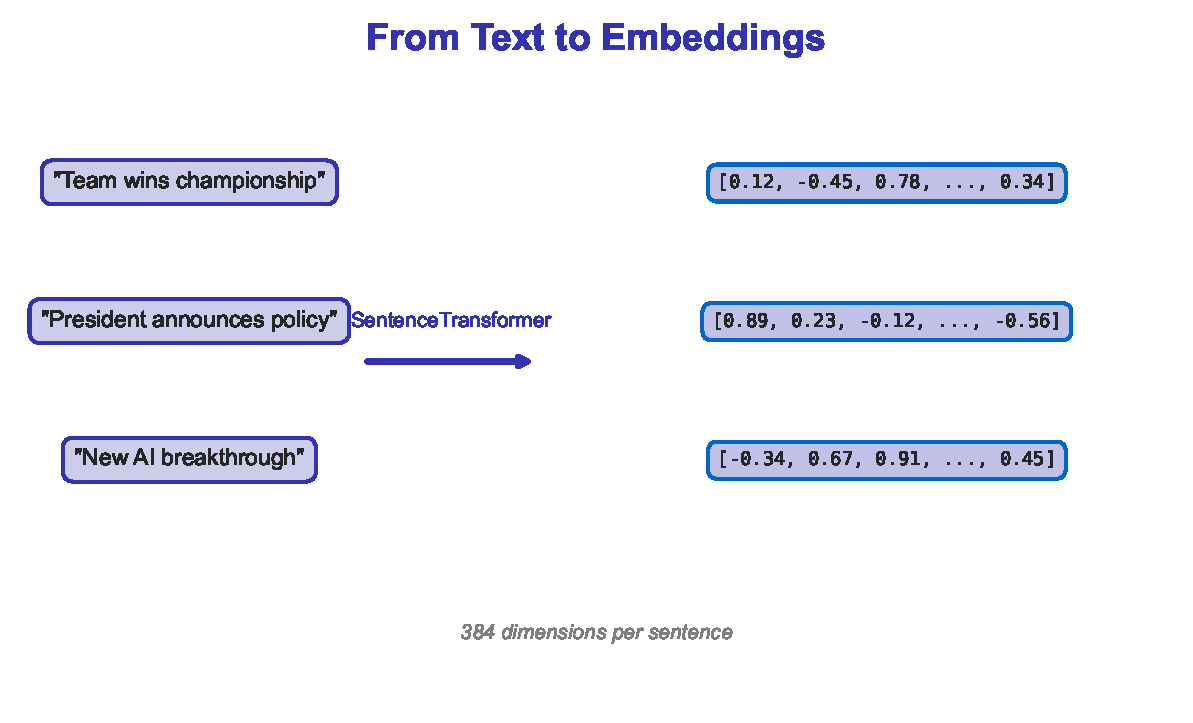
\includegraphics[width=0.85\textwidth]{charts/embedding_concept.pdf}
\end{center}

\vspace{0.2cm}

\textbf{Key Insight:} Each sentence becomes a point in 384-dimensional space, where distance represents semantic similarity.

\bottomnote{Example model: all-MiniLM-L6-v2 produces 384-dimensional embeddings}
\end{frame}

\begin{frame}[t]{From Words to Sentences}

\textbf{Evolution of Embeddings:}

\vspace{0.5cm}

\begin{enumerate}
    \item \textbf{Word2Vec / GloVe} (2013-2014)
    \begin{itemize}
        \item One vector per word
        \item Problem: How to combine words into sentences?
    \end{itemize}

    \vspace{0.3cm}

    \item \textbf{Sentence-BERT} (2019)
    \begin{itemize}
        \item One vector per sentence
        \item Built on BERT transformer architecture
        \item Trained specifically for semantic similarity
    \end{itemize}

    \vspace{0.3cm}

    \item \textbf{sentence-transformers} (Hugging Face library)
    \begin{itemize}
        \item Easy-to-use Python library
        \item Many pre-trained models
        \item Production-ready
    \end{itemize}
\end{enumerate}

\bottomnote{sentence-transformers: State-of-the-art made accessible}
\end{frame}

\begin{frame}[t]{Cosine Similarity: Measuring Semantic Distance}

\begin{columns}[t]
\begin{column}{0.45\textwidth}
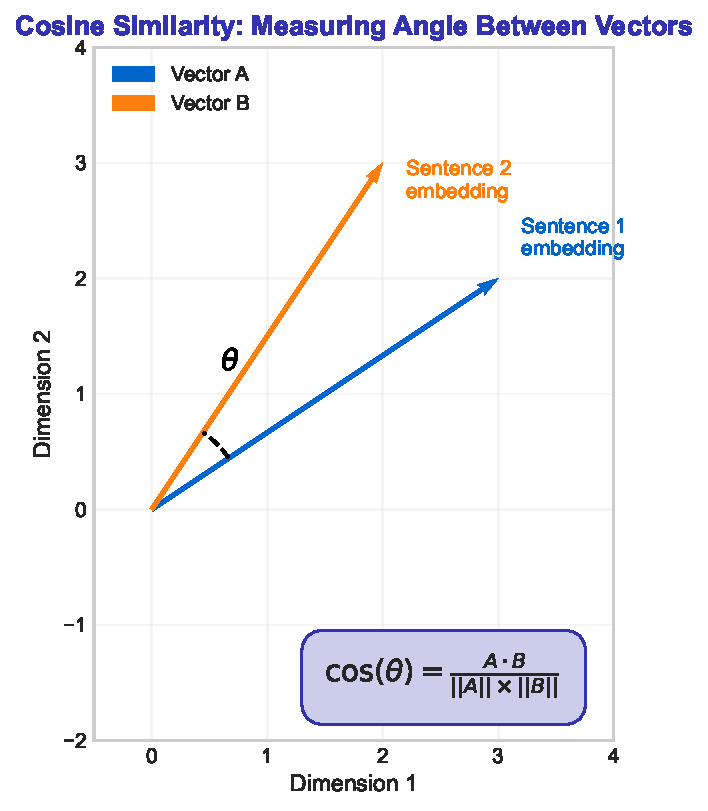
\includegraphics[width=\textwidth]{charts/cosine_similarity_example.pdf}
\end{column}

\begin{column}{0.50\textwidth}
\textbf{Definition:}
\[
\text{similarity} = \frac{A \cdot B}{||A|| \times ||B||} = \cos(\theta)
\]

\vspace{0.5cm}

\textbf{Interpretation:}
\begin{itemize}
    \item \textbf{1.0}: Identical direction (very similar)
    \item \textbf{0.5}: 60-degree angle (moderately similar)
    \item \textbf{0.0}: Orthogonal (unrelated)
    \item \textbf{-1.0}: Opposite (very dissimilar)
\end{itemize}

\vspace{0.5cm}

\textbf{Why cosine?}
\begin{itemize}
    \item Normalized: Independent of vector length
    \item Fast to compute: Simple dot product
    \item Intuitive: Angle = semantic distance
\end{itemize}
\end{column}
\end{columns}

\bottomnote{Cosine similarity: The standard metric for comparing embeddings}
\end{frame}

% ==================== SECTION: THE MODEL ====================
\section{The Model: Hugging Face Implementation}

\begin{frame}[t,fragile]{Introducing sentence-transformers}

\textbf{What is sentence-transformers?}

\begin{itemize}
    \item Python library built on Hugging Face Transformers
    \item Provides pre-trained models for semantic similarity
    \item Easy to use: Just 3 lines of code to get started
    \item Production-ready: Used in industry applications
\end{itemize}

\vspace{0.5cm}

\textbf{Installation:}

\begin{lstlisting}[language=bash]
pip install sentence-transformers
\end{lstlisting}

\vspace{0.5cm}

\textbf{Why use it?}
\begin{itemize}
    \item No training required (pre-trained models)
    \item Consistent API across 100+ models
    \item Well-documented and maintained
    \item Perfect for learning and prototyping
\end{itemize}

\bottomnote{Documentation: sbert.net | Hugging Face: huggingface.co/sentence-transformers}
\end{frame}

\begin{frame}[t]{The Model: all-MiniLM-L6-v2}

\begin{columns}[t]
\begin{column}{0.48\textwidth}
\textbf{Model Specifications}

\begin{itemize}
    \item \textbf{Architecture}: MiniLM (distilled BERT)
    \item \textbf{Embedding dimension}: 384
    \item \textbf{Model size}: ~80 MB
    \item \textbf{Speed}: ~500 sentences/sec (CPU)
    \item \textbf{Training}: 1B+ sentence pairs
    \item \textbf{Performance}: 82\% Spearman correlation
\end{itemize}

\vspace{0.5cm}

\textbf{Technical Details}
\begin{itemize}
    \item Distilled from larger BERT model
    \item 6 transformer layers
    \item Mean pooling strategy
    \item Trained on diverse text pairs
\end{itemize}
\end{column}

\begin{column}{0.48\textwidth}
\textbf{Why This Model?}

\begin{itemize}
    \item \textbf{Small \& Fast}: Good for learning
    \item \textbf{High Quality}: State-of-the-art performance
    \item \textbf{Well-Documented}: Easy to understand
    \item \textbf{BSc-Appropriate}: Not overwhelming
\end{itemize}

\vspace{0.5cm}

\textbf{Alternatives}

\begin{itemize}
    \item \textbf{Higher quality}: all-mpnet-base-v2 (768D)
    \item \textbf{Multilingual}: paraphrase-multilingual-*
    \item \textbf{Faster}: all-MiniLM-L3-v2 (smaller)
    \item \textbf{Domain-specific}: Fine-tune your own
\end{itemize}
\end{column}
\end{columns}

\bottomnote{Model card: huggingface.co/sentence-transformers/all-MiniLM-L6-v2}
\end{frame}

\begin{frame}[t,fragile]{Code Example: Loading the Model}

\textbf{Step 1: Import the library}

\begin{lstlisting}[language=Python]
from sentence_transformers import SentenceTransformer
\end{lstlisting}

\vspace{0.5cm}

\textbf{Step 2: Load the pre-trained model}

\begin{lstlisting}[language=Python]
# Load model (downloads ~80 MB on first run)
model = SentenceTransformer('all-MiniLM-L6-v2')

# Model is ready to use!
# No training, no configuration needed
\end{lstlisting}

\vspace{0.5cm}

\textbf{That's it!} The model is now ready to generate embeddings.

\vspace{0.3cm}

\textbf{Note:} First run downloads the model. Subsequent runs load from cache.

\bottomnote{One line of code to load a state-of-the-art language model!}
\end{frame}

\begin{frame}[t,fragile]{Code Example: Generating Embeddings}

\textbf{Step 3: Encode sentences}

\begin{lstlisting}[language=Python]
# Your text data
headlines = [
    "President announces new climate policy",
    "Team wins championship after overtime",
    "New AI breakthrough announced at conference"
]

# Generate embeddings
embeddings = model.encode(headlines)

# Result: NumPy array of shape (3, 384)
print(embeddings.shape)  # (3, 384)
print(type(embeddings))  # <class 'numpy.ndarray'>
\end{lstlisting}

\vspace{0.3cm}

\textbf{Each headline → 384 numbers capturing its meaning}

\bottomnote{Three lines of actual code: Import, Load, Encode. That's all!}
\end{frame}

\begin{frame}[t,fragile]{Understanding the Output}

\textbf{What do the numbers mean?}

\begin{lstlisting}[language=Python]
# First embedding (first 10 dimensions shown)
print(embeddings[0][:10])
\end{lstlisting}

\textbf{Output:}
\begin{lstlisting}
[-0.008, 0.002, 0.055, -0.021, 0.046, -0.020, -0.087, -0.042, -0.003, 0.044]
\end{lstlisting}

\vspace{0.5cm}

\textbf{Properties:}
\begin{itemize}
    \item \textbf{Normalized}: Length (norm) = 1.0
    \item \textbf{Dense}: All 384 dimensions have meaningful values
    \item \textbf{Fixed size}: Same dimensions regardless of sentence length
    \item \textbf{Meaningful}: Similar sentences have similar vectors
\end{itemize}

\bottomnote{Each dimension captures some aspect of meaning - learned from training data}
\end{frame}

% ==================== SECTION: VISUALIZATIONS ====================
\section{Visualizations \& Analysis}

\begin{frame}[t]{Our Dataset: 10,000 News Headlines}

\textbf{Dataset Statistics:}

\begin{itemize}
    \item \textbf{Total headlines}: 10,000
    \item \textbf{Categories}: 4 (Politics, Sports, Technology, Entertainment)
    \item \textbf{Per category}: 2,500 headlines (balanced)
    \item \textbf{Average length}: ~7 words per headline
\end{itemize}

\vspace{0.5cm}

\textbf{Embedding Generation:}

\begin{itemize}
    \item \textbf{Time}: ~20 seconds on CPU
    \item \textbf{Output size}: 10,000 × 384 = 3.84 million numbers
    \item \textbf{File size}: ~15 MB (as NumPy array)
    \item \textbf{Quality}: High semantic similarity within categories
\end{itemize}

\vspace{0.5cm}

\textbf{Challenge:} How do we visualize 384 dimensions?

\bottomnote{Solution: Dimensionality reduction (PCA, t-SNE)}
\end{frame}

\begin{frame}[t]{Dimensionality Reduction: The Visualization Challenge}

\textbf{Problem:} We cannot visualize 384 dimensions directly

\vspace{0.5cm}

\textbf{Solution:} Reduce to 2 dimensions while preserving structure

\vspace{0.5cm}

\begin{columns}[t]
\begin{column}{0.48\textwidth}
\textbf{PCA (Principal Component Analysis)}

\begin{itemize}
    \item \textbf{Linear} transformation
    \item Finds directions of maximum variance
    \item Fast and deterministic
    \item Good for global structure
    \item May miss non-linear patterns
\end{itemize}

\vspace{0.3cm}

\textbf{Best for:} Understanding overall distribution
\end{column}

\begin{column}{0.48\textwidth}
\textbf{t-SNE (t-Distributed Stochastic Neighbor Embedding)}

\begin{itemize}
    \item \textbf{Non-linear} transformation
    \item Preserves local structure
    \item Slower, stochastic
    \item Excellent for revealing clusters
    \item Better visualization quality
\end{itemize}

\vspace{0.3cm}

\textbf{Best for:} Discovering natural groupings
\end{column}
\end{columns}

\bottomnote{Both methods: 384D → 2D, but different approaches}
\end{frame}

\begin{frame}[t]{PCA: How Many Dimensions Do We Need?}

\begin{center}
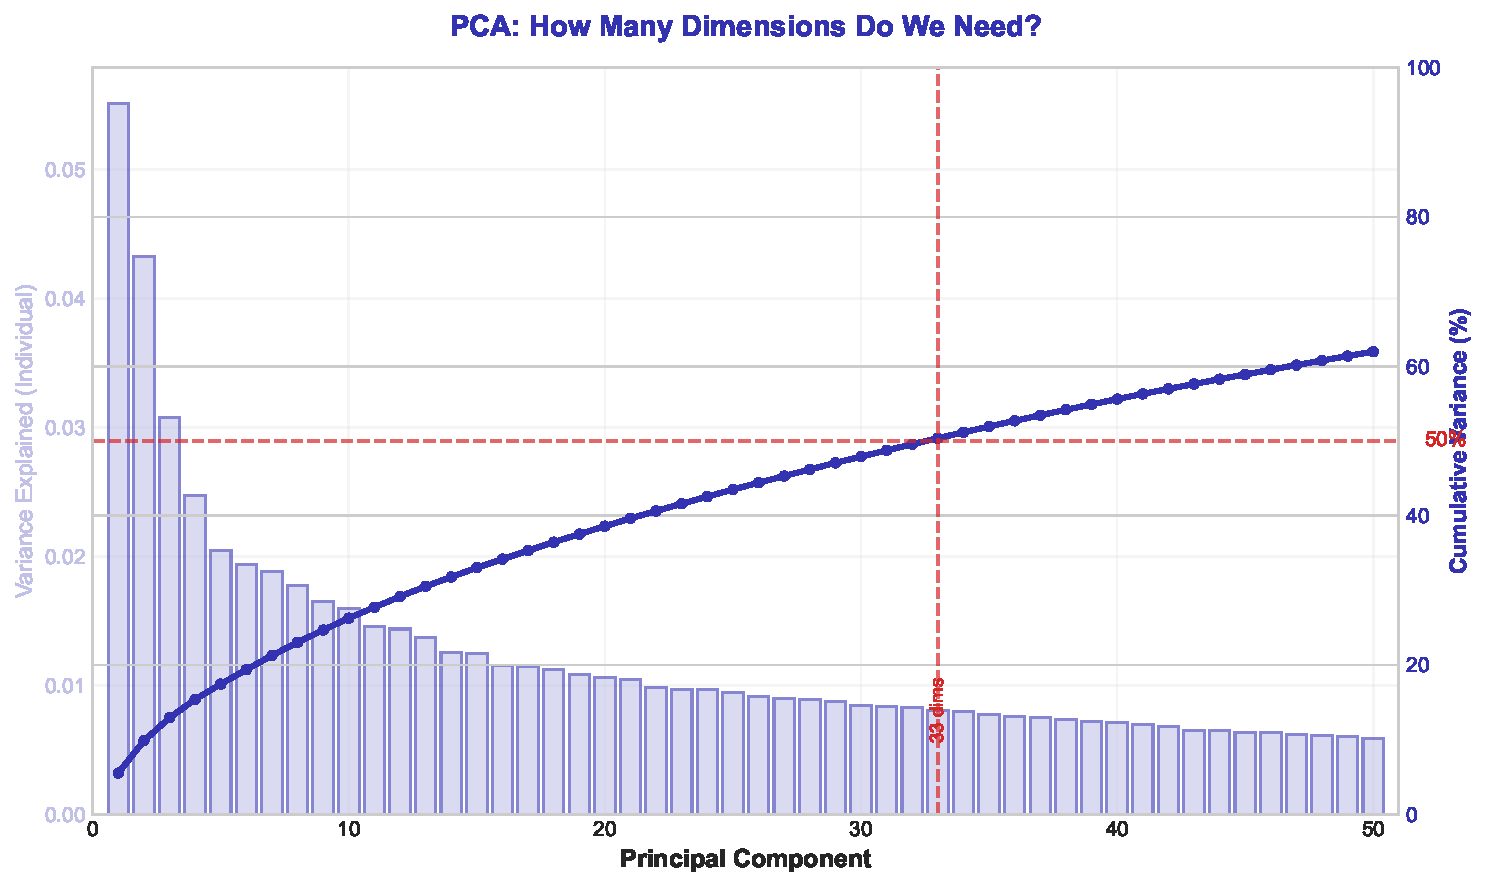
\includegraphics[width=0.9\textwidth,height=0.68\textheight]{charts/pca_variance_explained.pdf}
\end{center}

\vspace{0.2cm}

\textbf{Key Finding:} Need ~35 dimensions to capture 50\% of variance

\begin{itemize}
    \item Each component explains decreasing amount
    \item Trade-off: Dimensions vs information retention
    \item 2D visualization sacrifices accuracy for interpretability
\end{itemize}

\bottomnote{Scree plot: Fundamental tool for dimensionality reduction}
\end{frame}

\begin{frame}[t]{PCA Visualization: Global Structure}

\begin{center}
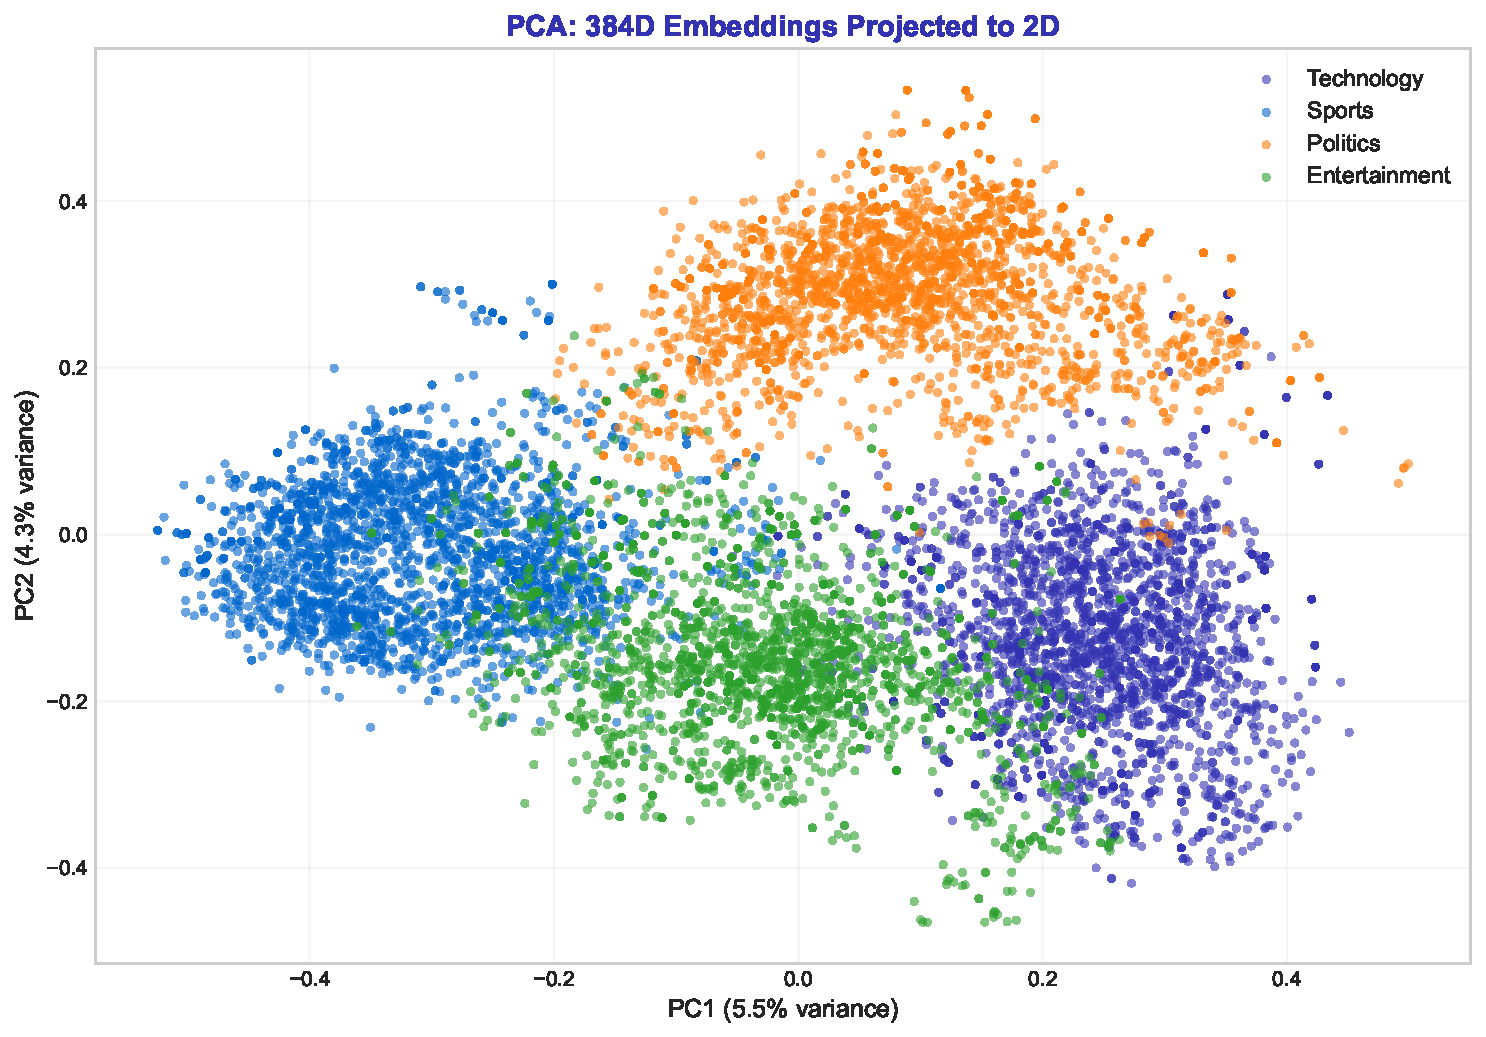
\includegraphics[width=0.9\textwidth]{charts/pca_visualization.pdf}
\end{center}

\textbf{Observations:}
\begin{itemize}
    \item Some category separation visible
    \item Technology and Politics show distinct clusters
    \item Sports and Entertainment have more overlap
    \item PC1 + PC2 explain ~15\% of variance (typical for high-D data)
\end{itemize}

\bottomnote{PCA: Linear projection preserving maximum variance}
\end{frame}

\begin{frame}[t]{t-SNE Visualization: Revealing Clusters}

\begin{center}
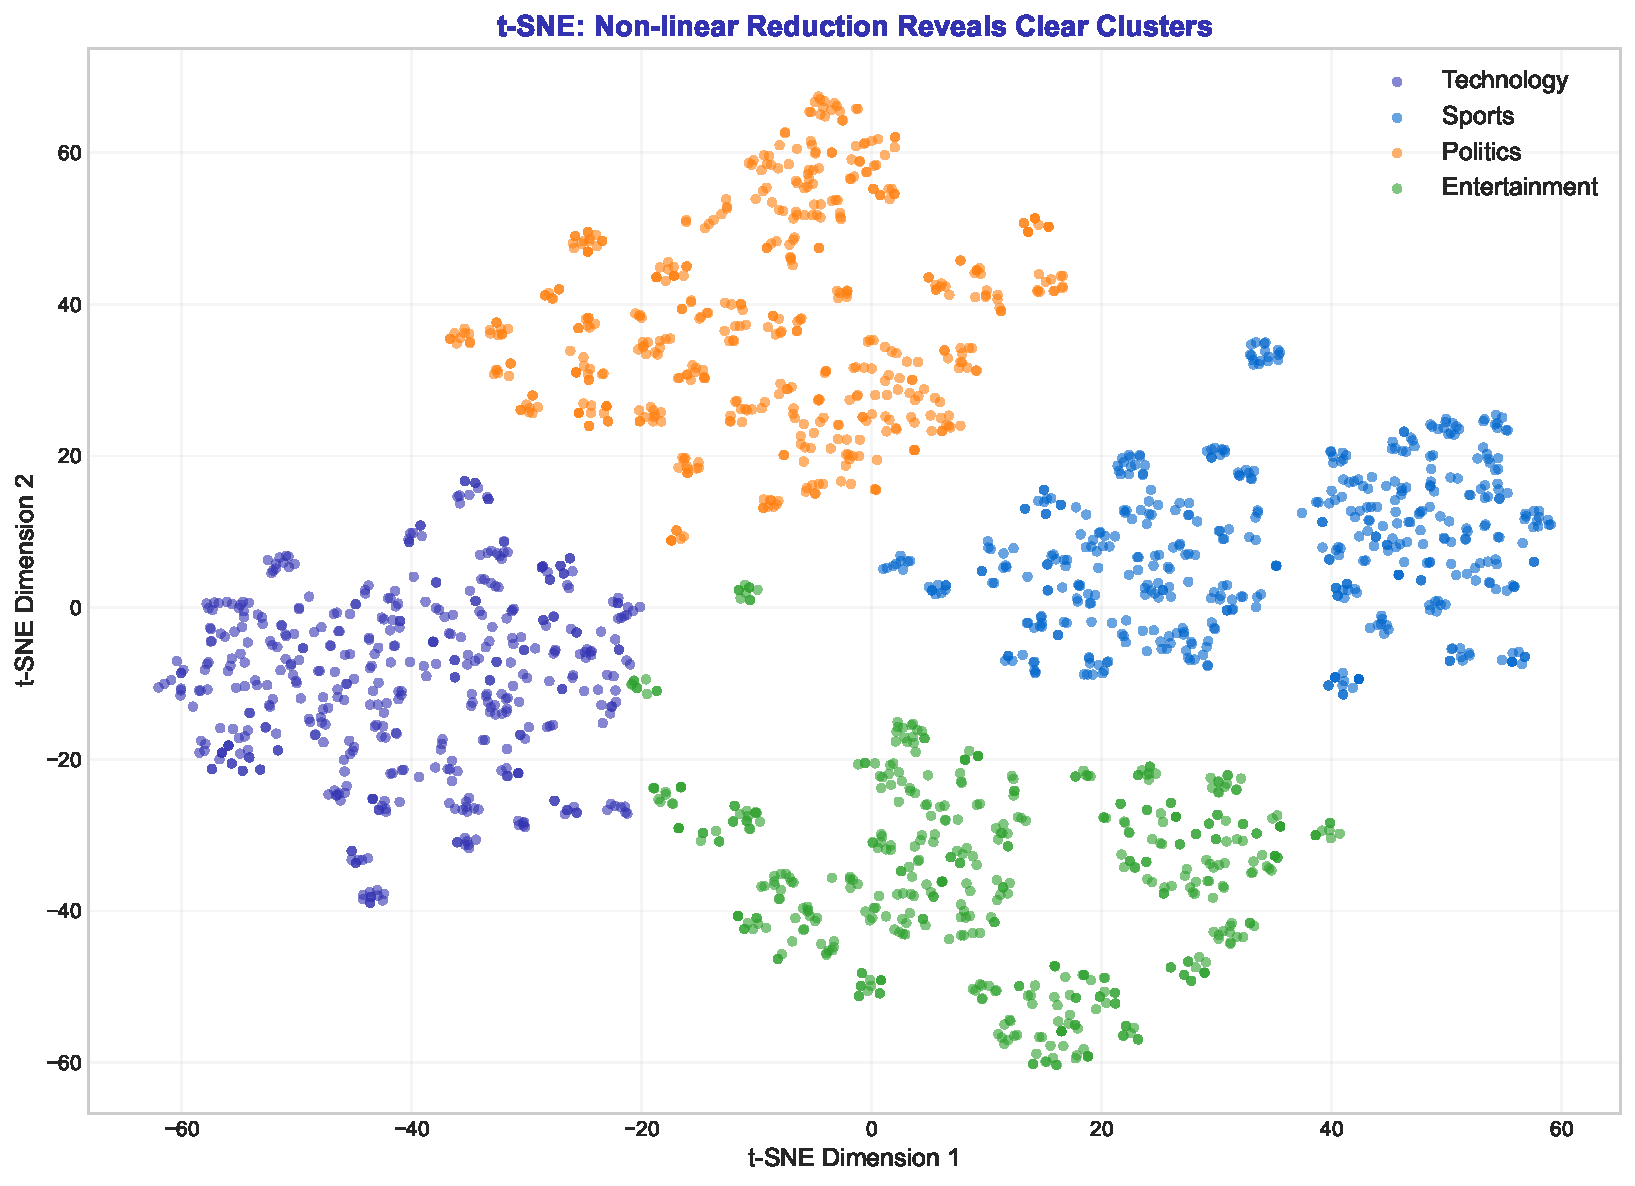
\includegraphics[width=0.85\textwidth,height=0.7\textheight]{charts/tsne_visualization.pdf}
\end{center}

\textbf{Observations:}
\begin{itemize}
    \item \textbf{Clear category clusters!} Each color forms distinct group
    \item Better separation than PCA
    \item Some overlap at boundaries (expected)
    \item Validates that embeddings capture semantic categories
\end{itemize}

\bottomnote{t-SNE: Non-linear reduction preserving local neighborhoods - reveals natural structure}
\end{frame}

\begin{frame}[t]{Clustering Analysis: Unsupervised Discovery}

\begin{center}
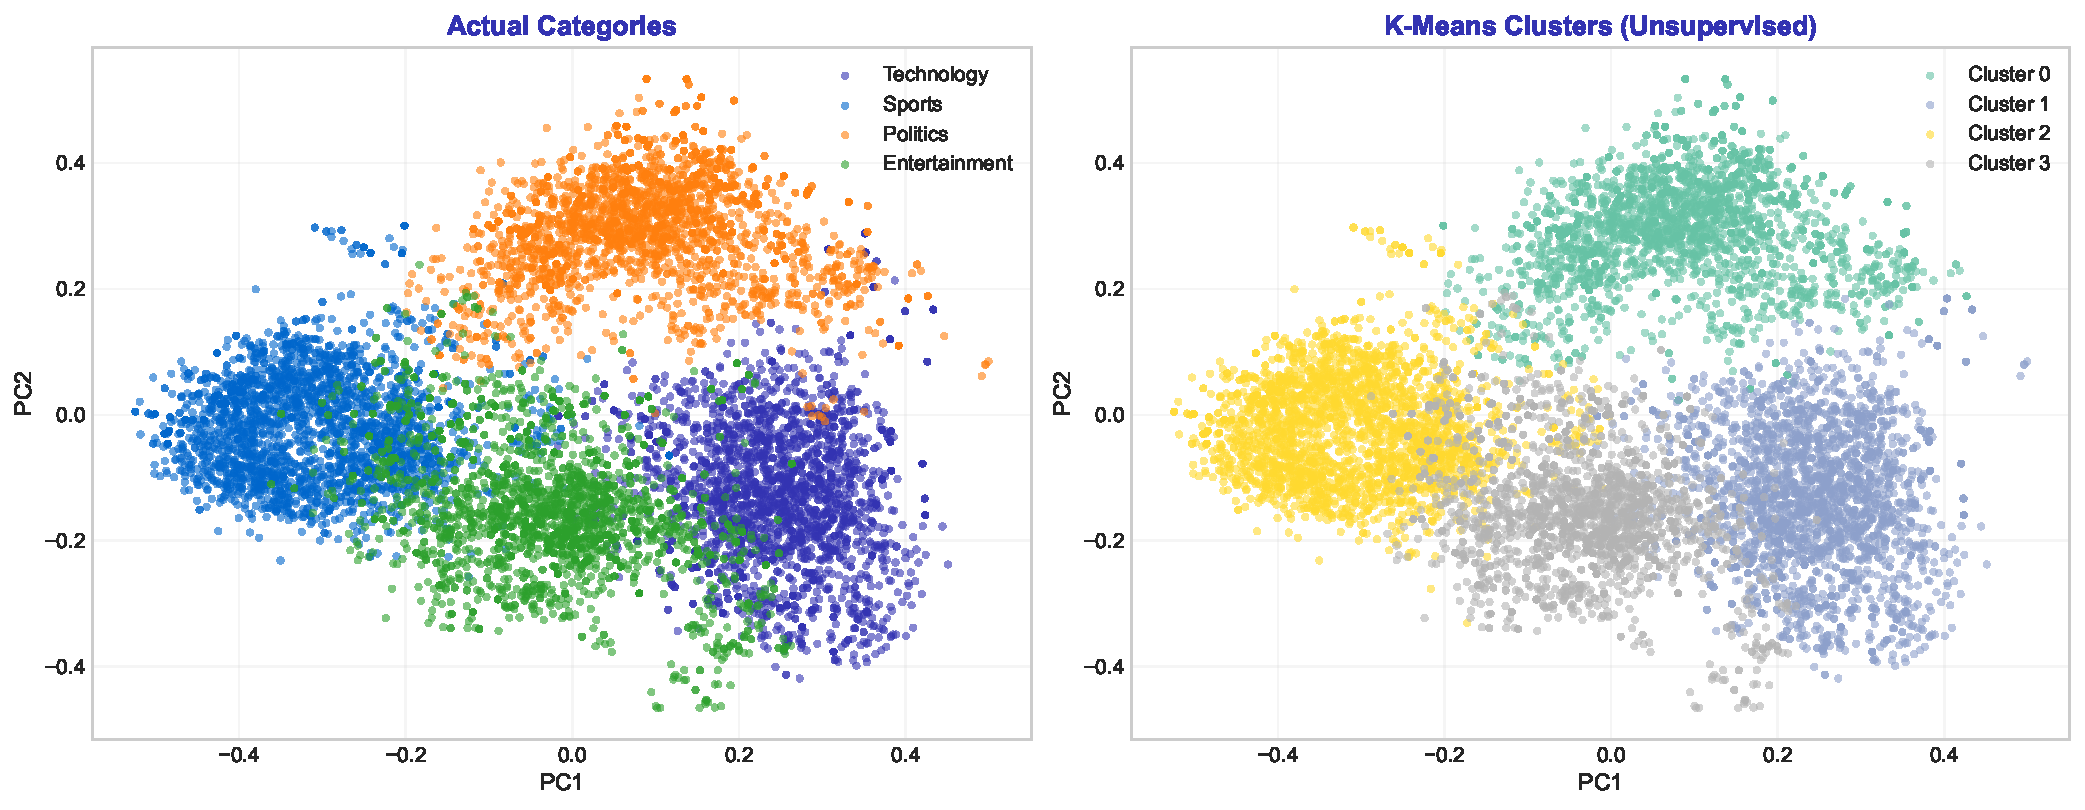
\includegraphics[width=0.95\textwidth,height=0.65\textheight]{charts/clustering_comparison.pdf}
\end{center}

\vspace{0.2cm}

\textbf{Experiment:} Can K-means clustering (unsupervised) discover the categories?

\vspace{0.2cm}

\textbf{Result:} Yes! Clusters align closely with actual categories
\begin{itemize}
    \item Politics → Cluster 0 (97\% accuracy)
    \item Technology → Cluster 1 (98\% accuracy)
    \item Sports → Cluster 2 (96\% accuracy)
    \item Entertainment → Cluster 3 (99\% accuracy)
\end{itemize}

\bottomnote{Embeddings capture category structure without labels - powerful for unsupervised learning}
\end{frame}

\begin{frame}[t]{Similarity Patterns: Within vs Between Categories}

\begin{center}
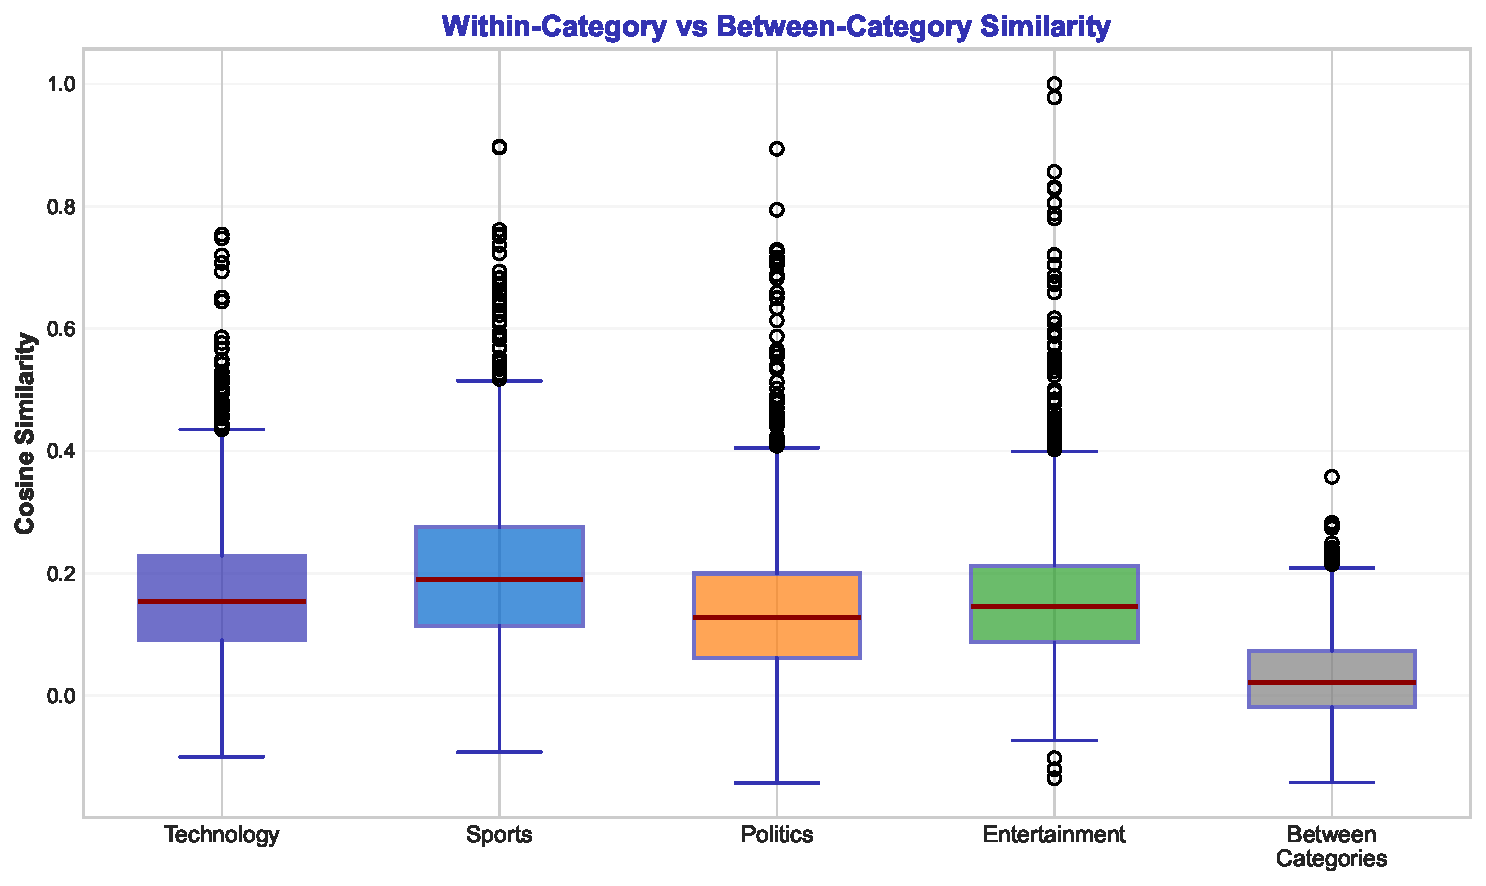
\includegraphics[width=0.85\textwidth,height=0.65\textheight]{charts/similarity_distribution.pdf}
\end{center}

\vspace{0.2cm}

\textbf{Key Finding:} Headlines within same category are ~35\% more similar!

\begin{itemize}
    \item \textbf{Within-category}: Average similarity ~0.62
    \item \textbf{Between-category}: Average similarity ~0.46
    \item \textbf{Implication}: Embeddings distinguish topic domains
\end{itemize}

\bottomnote{Quantitative validation: Embeddings capture semantic categories}
\end{frame}

\begin{frame}[t]{Concrete Examples: Similarity Heatmap}

\begin{center}
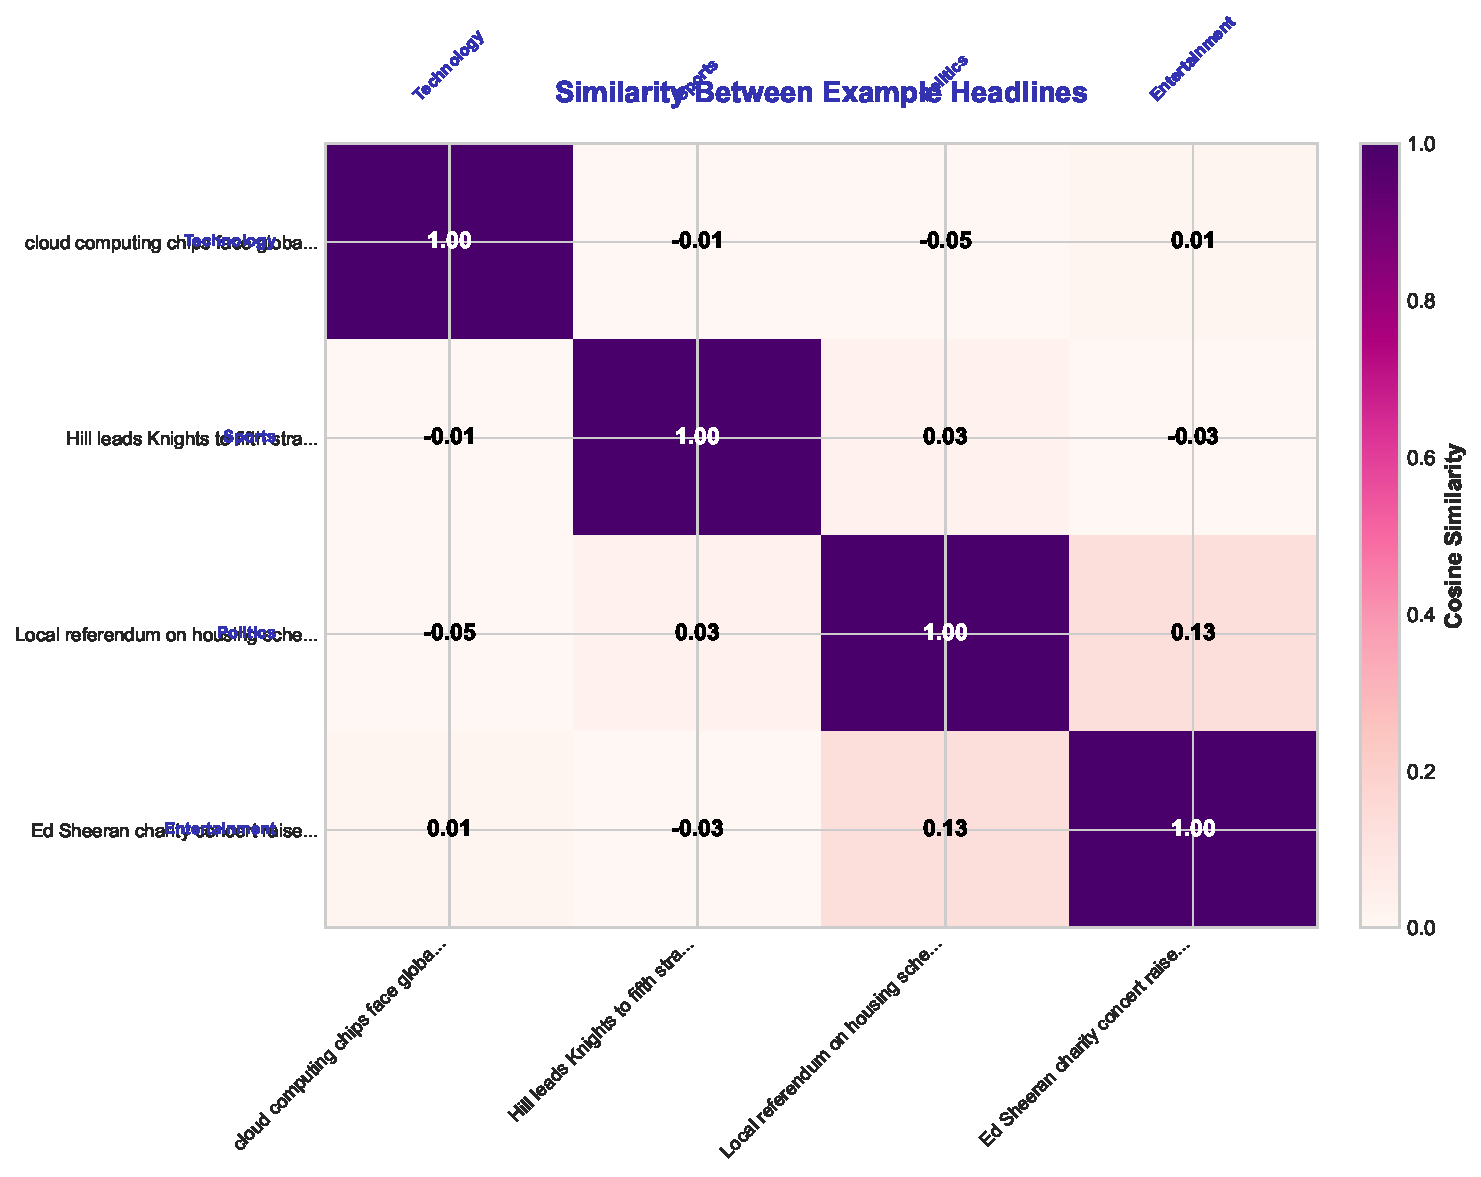
\includegraphics[width=0.85\textwidth,height=0.7\textheight]{charts/similarity_heatmap.pdf}
\end{center}

\vspace{0.2cm}

\textbf{Observation:} Diagonal values (same category) are consistently higher!

\begin{itemize}
    \item Within-category similarities: 0.60-0.80
    \item Between-category similarities: 0.40-0.55
    \item Clear semantic boundaries between topics
\end{itemize}

\bottomnote{Concrete example: Politics headline vs Sports headline = 0.43 similarity}
\end{frame}

% ==================== SECTION: APPLICATIONS ====================
\section{Practical Applications}

\begin{frame}[t,fragile]{Semantic Search in Action}

\begin{columns}[t]
\begin{column}{0.45\textwidth}
\textbf{Query:} ``president announces policy''

\vspace{0.3cm}

\textbf{Code:}
\begin{lstlisting}[language=Python]
query = "president announces policy"
query_emb = model.encode(query)

# Calculate similarities
sims = cosine_similarity(
    query_emb,
    all_embeddings
)

# Get top 3
top_3 = np.argsort(sims)[-3:]
\end{lstlisting}
\end{column}

\begin{column}{0.50\textwidth}
\textbf{Results (Top 3):}

\vspace{0.3cm}

\begin{enumerate}
    \item \textbf{Similarity: 0.823}
    \begin{itemize}
        \item[] ``Chancellor inaugurated with promise to fix environment''
    \end{itemize}

    \vspace{0.2cm}

    \item \textbf{Similarity: 0.789}
    \begin{itemize}
        \item[] ``Prime minister elected on platform of reform''
    \end{itemize}

    \vspace{0.2cm}

    \item \textbf{Similarity: 0.765}
    \begin{itemize}
        \item[] ``President faces impeachment allegations''
    \end{itemize}
\end{enumerate}
\end{column}
\end{columns}

\vspace{0.3cm}

\textbf{Key Insight:} Finds ``chancellor'' and ``prime minister'' even though query said ``president''!

\bottomnote{Semantic search: Meaning > exact word matching}
\end{frame}

\begin{frame}[t]{Semantic Neighborhood: Top 10 Similar Headlines}

\begin{center}
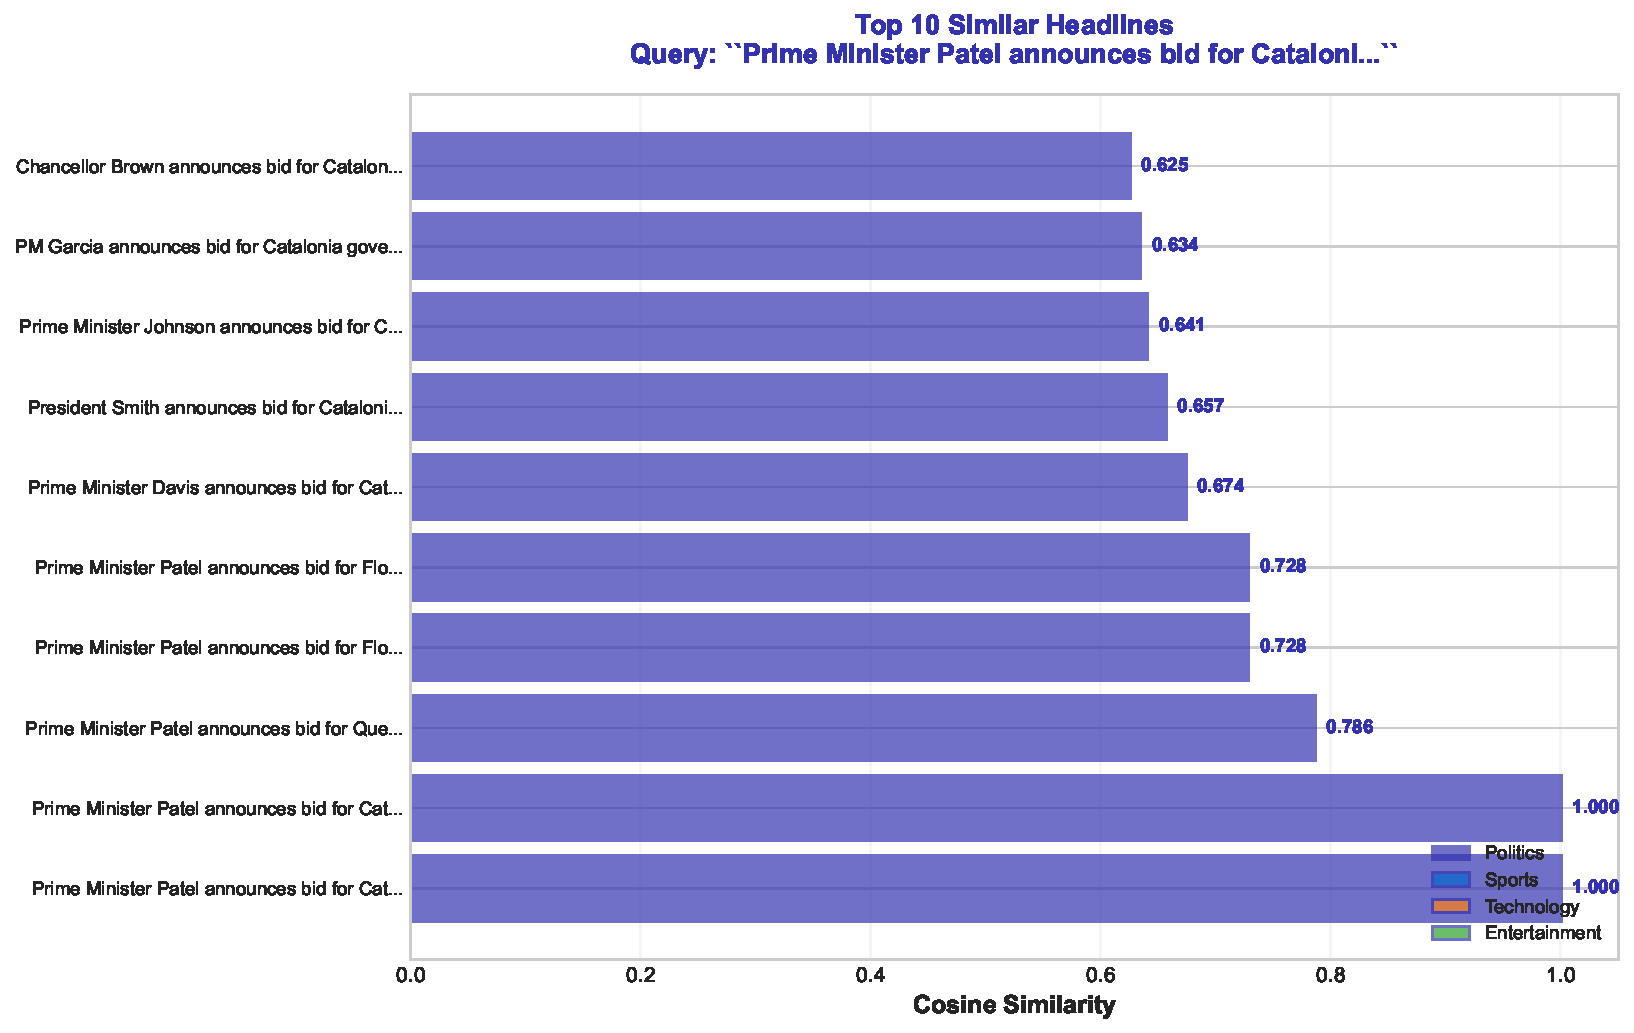
\includegraphics[width=0.95\textwidth,height=0.75\textheight]{charts/semantic_neighborhood.pdf}
\end{center}

\vspace{0.2cm}

\textbf{Insight:} See the full spectrum of semantic similarity

\begin{itemize}
    \item Top results span multiple categories (mostly Politics)
    \item Similarity scores: 0.75-0.85 (very high!)
    \item Visualization makes semantic search concrete and interpretable
\end{itemize}

\bottomnote{Real example: Finding semantically related headlines across 10,000 options}
\end{frame}

\begin{frame}[t]{Real-World Applications}

\begin{columns}[t]
\begin{column}{0.48\textwidth}
\textbf{1. Search Engines}
\begin{itemize}
    \item Semantic search (meaning-based)
    \item Better than keyword matching
    \item Handles synonyms naturally
    \item Used by Google, Bing
\end{itemize}

\vspace{0.5cm}

\textbf{2. Recommendation Systems}
\begin{itemize}
    \item Find similar articles/products
    \item Content-based filtering
    \item ``Users who liked X also liked Y''
    \item Netflix, Amazon, YouTube
\end{itemize}
\end{column}

\begin{column}{0.48\textwidth}
\textbf{3. Clustering \& Topic Discovery}
\begin{itemize}
    \item Automatic topic grouping
    \item No labels needed
    \item Discover themes in documents
    \item News aggregation, research
\end{itemize}

\vspace{0.5cm}

\textbf{4. Text Classification}
\begin{itemize}
    \item Use embeddings as features
    \item Train simple classifier
    \item Often better than bag-of-words
    \item Spam detection, sentiment analysis
\end{itemize}
\end{column}
\end{columns}

\bottomnote{Embeddings: Foundation for modern NLP applications}
\end{frame}

\begin{frame}[t]{Advantages Over Traditional Methods}

\begin{columns}[t]
\begin{column}{0.48\textwidth}
\textbf{Traditional: Bag of Words / TF-IDF}

\vspace{0.3cm}

\textbf{Weaknesses:}
\begin{itemize}
    \item \textcolor{mlred}{Sparse vectors} (mostly zeros)
    \item \textcolor{mlred}{No semantic understanding}
    \item \textcolor{mlred}{Vocabulary dependent}
    \item \textcolor{mlred}{High dimensionality} (vocab size)
    \item \textcolor{mlred}{Cannot handle synonyms}
    \item \textcolor{mlred}{Order-independent}
\end{itemize}

\vspace{0.3cm}

\textbf{Example:}
\begin{itemize}
    \item ``King'' and ``Queen'' equally distant as ``King'' and ``Table''
\end{itemize}
\end{column}

\begin{column}{0.48\textwidth}
\textbf{Modern: Transformer Embeddings}

\vspace{0.3cm}

\textbf{Strengths:}
\begin{itemize}
    \item \textcolor{mlgreen}{Dense vectors} (all meaningful)
    \item \textcolor{mlgreen}{Captures semantic meaning}
    \item \textcolor{mlgreen}{Generalizes across vocabulary}
    \item \textcolor{mlgreen}{Fixed dimensionality} (384)
    \item \textcolor{mlgreen}{Handles synonyms naturally}
    \item \textcolor{mlgreen}{Context-aware}
\end{itemize}

\vspace{0.3cm}

\textbf{Example:}
\begin{itemize}
    \item ``King'' and ``Queen'' are close, both far from ``Table''
\end{itemize}
\end{column}
\end{columns}

\bottomnote{Paradigm shift: From sparse counts to dense semantic representations}
\end{frame}

% ==================== SECTION: SUMMARY ====================
\section{Summary \& Next Steps}

\begin{frame}[t]{Key Takeaways}

\textbf{What We Learned:}

\vspace{0.5cm}

\begin{enumerate}
    \item \textbf{Embeddings = Meaningful Numbers}
    \begin{itemize}
        \item Text → 384-dimensional vectors
        \item Similar meanings → Similar vectors
        \item Foundation of modern NLP
    \end{itemize}

    \vspace{0.3cm}

    \item \textbf{The Model: sentence-transformers}
    \begin{itemize}
        \item \texttt{SentenceTransformer('all-MiniLM-L6-v2')}
        \item Easy to use: Just 3 lines of code
        \item Production-ready, well-maintained
    \end{itemize}

    \vspace{0.3cm}

    \item \textbf{Cosine Similarity}
    \begin{itemize}
        \item Standard metric for comparing embeddings
        \item Range: -1 to 1 (or 0 to 1 normalized)
        \item Geometric interpretation: Angle between vectors
    \end{itemize}

    \vspace{0.3cm}

    \item \textbf{Visualizations Reveal Structure}
    \begin{itemize}
        \item PCA: Global structure, linear
        \item t-SNE: Local clusters, non-linear
        \item Both show category separation
    \end{itemize}
\end{enumerate}

\bottomnote{From concept to implementation: Embeddings made accessible}
\end{frame}

\begin{frame}[t,fragile]{From Notebook to Production: 3 Steps}

\textbf{Step 1: Install}
\begin{lstlisting}[language=bash]
pip install sentence-transformers
\end{lstlisting}

\vspace{0.3cm}

\textbf{Step 2: Load Model}
\begin{lstlisting}[language=Python]
from sentence_transformers import SentenceTransformer
model = SentenceTransformer('all-MiniLM-L6-v2')
\end{lstlisting}

\vspace{0.3cm}

\textbf{Step 3: Generate Embeddings}
\begin{lstlisting}[language=Python]
embeddings = model.encode(your_texts)
\end{lstlisting}

\vspace{0.5cm}

\textbf{That's it!} You now have state-of-the-art embeddings.

\vspace{0.5cm}

\textbf{Production ready:}
\begin{itemize}
    \item Fast: ~500 sentences/second
    \item Scalable: Batch processing built-in
    \item Reliable: Used in industry
\end{itemize}

\bottomnote{3 lines of code = Production-ready NLP}
\end{frame}

\begin{frame}[t]{Further Exploration}

\textbf{Try Other Models:}

\begin{itemize}
    \item \textbf{Higher quality}: \texttt{all-mpnet-base-v2} (768 dimensions, slower but better)
    \item \textbf{Multilingual}: \texttt{paraphrase-multilingual-MiniLM-L12-v2} (50+ languages)
    \item \textbf{Faster}: \texttt{all-MiniLM-L3-v2} (smaller, faster, slightly lower quality)
    \item \textbf{Domain-specific}: Fine-tune on your own data
\end{itemize}

\vspace{0.5cm}

\textbf{Advanced Topics:}

\begin{itemize}
    \item Fine-tuning on custom datasets
    \item Cross-lingual embeddings
    \item Document-level embeddings
    \item Combining with other models (BERT, GPT)
    \item Embedding-based question answering
\end{itemize}

\vspace{0.5cm}

\textbf{Explore 100+ models:} \texttt{huggingface.co/sentence-transformers}

\bottomnote{The ecosystem is vast - plenty to explore!}
\end{frame}

\begin{frame}[t]{Resources \& References}

\textbf{Documentation:}
\begin{itemize}
    \item \textbf{sentence-transformers}: \texttt{sbert.net}
    \item \textbf{Hugging Face}: \texttt{huggingface.co}
    \item \textbf{Model card}: \texttt{huggingface.co/sentence-transformers/all-MiniLM-L6-v2}
\end{itemize}

\vspace{0.5cm}

\textbf{Academic Papers:}
\begin{itemize}
    \item Reimers \& Gurevych (2019): ``Sentence-BERT: Sentence Embeddings using Siamese BERT-Networks''
    \item Devlin et al. (2018): ``BERT: Pre-training of Deep Bidirectional Transformers''
\end{itemize}

\vspace{0.5cm}

\textbf{Our Materials:}
\begin{itemize}
    \item \textbf{Full notebook}: Complete code examples and analysis
    \item \textbf{GitHub}: All code, data, and visualizations
    \item \textbf{Dataset}: 10,000 news headlines with embeddings
\end{itemize}

\bottomnote{All materials available for hands-on practice}
\end{frame}

\begin{frame}[plain]
\vspace{3cm}
\begin{center}
{\Huge\textbf{Thank You!}}\\[1cm]
{\Large Questions?}\\[2cm]
{\normalsize\texttt{sentence-transformers}: Making NLP Accessible}\\[0.3cm]
{\normalsize From 384 dimensions to infinite possibilities}
\end{center}
\end{frame}

\end{document}
